%% LyX 2.2.2 created this file.  For more info, see http://www.lyx.org/.
%% Do not edit unless you really know what you are doing.
\documentclass[9pt,twoside,english]{extarticle}
\usepackage[T1]{fontenc}
\usepackage[latin9]{inputenc}
\usepackage[letterpaper]{geometry}
\geometry{verbose,tmargin=3cm,bmargin=2cm,lmargin=2cm,rmargin=2cm,headheight=1cm,headsep=0.5cm,footskip=1cm}
\usepackage{color}
\definecolor{page_backgroundcolor}{rgb}{1, 1, 1}
\pagecolor{page_backgroundcolor}
\definecolor{document_fontcolor}{rgb}{0, 0, 0}
\color{document_fontcolor}
\usepackage{babel}
\usepackage{float}
\usepackage{amsmath}
\usepackage{amsthm}
\usepackage{graphicx}
\usepackage[unicode=true,pdfusetitle,
 bookmarks=true,bookmarksnumbered=false,bookmarksopen=false,
 breaklinks=false,pdfborder={0 0 1},backref=false,colorlinks=true]
 {hyperref}

\makeatletter

%%%%%%%%%%%%%%%%%%%%%%%%%%%%%% LyX specific LaTeX commands.
%% Because html converters don't know tabularnewline
\providecommand{\tabularnewline}{\\}

%%%%%%%%%%%%%%%%%%%%%%%%%%%%%% Textclass specific LaTeX commands.
\numberwithin{equation}{section}
\numberwithin{figure}{section}

\@ifundefined{showcaptionsetup}{}{%
 \PassOptionsToPackage{caption=false}{subfig}}
\usepackage{subfig}
\makeatother

\begin{document}

\title{\textbf{Project 02}\\
\textbf{Model Predictive Control}}

\author{\textbf{Prem Sagar S - AE14B021}}
\maketitle

\section{Formulation}

With usual notations, the control input plan is determined by optmising
the objective function:

\[
J=\sum_{i=1}^{p}\left(\hat{Y}_{k+i/k}-Y_{k+i}^{ref}\right)^{T}Q^{y}\left(\hat{Y}_{k+i/k}-Y_{k+i}^{ref}\right)+\sum_{j=0}^{m-1}u_{m+j}^{T}Q^{u}u_{m+j}
\]

The prediction at k+i time step can be written as:

\begin{eqnarray*}
\hat{Y}_{k+i/k} & = & CA^{i}\hat{X}_{k/k}+CA^{i-1}Bu_{k}+CA^{i-2}Bu_{k+1}+\ldots+CA^{0}Bu_{k+i-1}\\
 & = & CA^{i}\hat{X}_{k/k}+\begin{bmatrix}CA^{i-1}B & CA^{i-2}B & \ldots & CA^{0}B\end{bmatrix}\begin{bmatrix}u_{k}\\
u_{k+1}\\
\vdots\\
u_{k+i-1}
\end{bmatrix}\\
 & = & CA^{i}\hat{X}_{k/k}+CAB_{i}\begin{bmatrix}u_{k}\\
u_{k+1}\\
\vdots\\
u_{k+m-1}
\end{bmatrix}\\
 & = & CA^{i}\hat{X}_{k/k}+CAB_{i}U
\end{eqnarray*}

where,
\[
CAB_{i}=\begin{cases}
\begin{bmatrix}CA^{i-1}B & CA^{i-2}B & \ldots & CA^{0}B & 0 & 0 & \ldots & 0\end{bmatrix}_{1\times m} & i\leq m\\
\begin{bmatrix}CA^{i-1}B & CA^{i-2}B & \ldots & CA^{i-m+1}B & C\left(A^{0}+A^{1}+...+A^{(i-m)}\right)B\end{bmatrix}_{1\times m} & i>m
\end{cases}
\]

Using this, the objective function can be written in the form below
\[
J=\frac{1}{2}U^{T}HU+f^{T}U+K
\]

where,
\begin{eqnarray*}
H & = & \sum_{i=1}^{p}CAB_{i}^{T}Q^{y}CAB_{i}+\begin{bmatrix}Q^{u} & 0 & \cdots & 0\\
0 & Q^{u} & \cdots & 0\\
\vdots & \vdots & \ddots & 0\\
0 & 0 & \cdots & Q^{u}
\end{bmatrix}_{m\times m}\\
f & = & -\sum_{i=1}^{p}\hat{X}_{k/k}^{T}\left(A^{i}\right)^{T}C^{T}Q^{y}CAB_{i}+\sum_{i=1}^{p}\left(Y_{k+i}^{ref}\right)^{T}Q^{y}CAB_{i}
\end{eqnarray*}

\textbf{U }is then solved for using the matlab function quadprog.

To have a handle on the measurements being contorlled, the C matrix
can be premultipied with an appropriate identity matrix. For example,
to control first and last measurement,

\[
C=\begin{bmatrix}1 & 0 & 0\\
0 & 0 & 1
\end{bmatrix}C_{new}
\]


\section{Control System }

\begin{figure}[H]
\begin{centering}
\includegraphics[width=0.9\paperwidth]{MatlabMain/results/MPC.PNG}
\par\end{centering}
\caption{Schematic of Control on FCC}

\end{figure}

The above schematic shows the implementation of MPC in Simulink. (For
representative purpose only) The plant measurements are simulated
by solving the plant's differential equations. The measurement is
fed to the Kalman filter that works on the linearized model. The filtered
state estimate is fed to the controller which gives the optimal control
input to the plant. This goes on.

\section{Measurements with No Noise}

\subsection{Constant set-point profile}

\begin{table}[H]
\begin{centering}
\begin{tabular}{|c|c|}
\hline 
\textbf{Kalman Filter} & \textbf{Controller}\tabularnewline
\hline 
\hline 
$X_{0}=\begin{bmatrix}0.0472\\
-0.0576\\
-0.1655\\
-0.1065
\end{bmatrix}$ & p=7\tabularnewline
\hline 
$P_{0/0}=30000\times\begin{bmatrix}1 & 1 & 1 & 1\\
1 & 1 & 1 & 1\\
1 & 1 & 1 & 1\\
1 & 1 & 1 & 1
\end{bmatrix}$ & m=3\tabularnewline
\hline 
$Q=10e-3\times\begin{bmatrix}1 & 0 & 0 & 0\\
0 & 1 & 0 & 0\\
0 & 0 & 1 & 0\\
0 & 0 & 0 & 1
\end{bmatrix}$ & $Q_{y}=\begin{bmatrix}4 & 0 & 0\\
0 & 5 & 0\\
0 & 0 & 5
\end{bmatrix}$\tabularnewline
\hline 
$R=\begin{bmatrix}10 & 0 & 0\\
0 & 20 & 0\\
0 & 0 & 100
\end{bmatrix}$ & $Q_{u}=\begin{bmatrix}0.05 & 0\\
0 & 0.05
\end{bmatrix}$\tabularnewline
\hline 
\end{tabular}
\par\end{centering}
\caption{Tuned parameters}
\end{table}

\begin{figure}[H]
\begin{centering}
\subfloat[$C_{rc}$]{\begin{centering}
\includegraphics[scale=0.5]{\string"MatlabMain/results/No noise/Crc\string".pdf}
\par\end{centering}
}\subfloat[$O_{d}$]{\begin{centering}
\includegraphics[scale=0.5]{\string"MatlabMain/results/No noise/Od\string".pdf}
\par\end{centering}
}
\par\end{centering}
\begin{centering}
\subfloat[$T_{rg}$]{\begin{centering}
\includegraphics[scale=0.5]{\string"MatlabMain/results/No noise/Trg\string".pdf}
\par\end{centering}
}\subfloat[Inputs]{\begin{centering}
\includegraphics[scale=0.5]{\string"MatlabMain/results/No noise/inputs\string".pdf}
\par\end{centering}
}
\par\end{centering}
\caption{\textbf{\emph{Constant set-point profile}}\emph{ - }\textbf{\emph{Measurements
with No Noise: }}\emph{First state keeps increasing, while the other
two saturate with an offset from the set point}}
\end{figure}


\subsection{Non constant set-point profile}

\begin{table}[H]
\begin{centering}
\begin{tabular}{|c|c|}
\hline 
\textbf{Kalman Filter} & \textbf{Controller}\tabularnewline
\hline 
\hline 
$X_{0}=\begin{bmatrix}0.0472\\
-0.0576\\
-0.1655\\
-0.1065
\end{bmatrix}$ & p=7\tabularnewline
\hline 
$P_{0/0}=30000\times\begin{bmatrix}1 & 1 & 1 & 1\\
1 & 1 & 1 & 1\\
1 & 1 & 1 & 1\\
1 & 1 & 1 & 1
\end{bmatrix}$ & m=3\tabularnewline
\hline 
$Q=10e-3\times\begin{bmatrix}1 & 0 & 0 & 0\\
0 & 1 & 0 & 0\\
0 & 0 & 1 & 0\\
0 & 0 & 0 & 1
\end{bmatrix}$ & $Q_{y}=\begin{bmatrix}4 & 0 & 0\\
0 & 5 & 0\\
0 & 0 & 5
\end{bmatrix}$\tabularnewline
\hline 
$R=\begin{bmatrix}10 & 0 & 0\\
0 & 20 & 0\\
0 & 0 & 100
\end{bmatrix}$ & $Q_{u}=\begin{bmatrix}0.05 & 0\\
0 & 0.05
\end{bmatrix}$\tabularnewline
\hline 
\end{tabular}
\par\end{centering}
\caption{Tuned parameters}
\end{table}

\begin{figure}[H]
\begin{centering}
\subfloat[$C_{rc}$]{\begin{centering}
\includegraphics[scale=0.6]{\string"MatlabMain/results/No noise/Non const sp/Crc\string".pdf}
\par\end{centering}
}\subfloat[$O_{d}$]{\begin{centering}
\includegraphics[scale=0.6]{\string"MatlabMain/results/No noise/Non const sp/Od\string".pdf}
\par\end{centering}
}
\par\end{centering}
\centering{}\subfloat[$T_{rg}$]{\begin{centering}
\includegraphics[scale=0.6]{\string"MatlabMain/results/No noise/Non const sp/Trg\string".pdf}
\par\end{centering}
}\subfloat[Inputs]{\begin{centering}
\includegraphics[scale=0.6]{\string"MatlabMain/results/No noise/Non const sp/inputs\string".pdf}
\par\end{centering}
}\caption{\textbf{\emph{Non Constant set-point profile - Measurements with no
noise: }}\emph{The behaviour is same as in previous case. The saturation
value for the last two states have reduced. The saturated states stay
that way and don't seem to make an effort to reach the set point.}}
\end{figure}


\section{Measurements with Gaussian Noise}

Gaussian noise $N(0,\sigma)$ is added to the plant generated measurements. 

\[
\sigma=\begin{bmatrix}0.001 & 0 & 0\\
0 & 0.001 & 0\\
0 & 0 & 1.5
\end{bmatrix}
\]


\subsection{Constant set-point profile}

\begin{table}[H]
\begin{centering}
\begin{tabular}{|c|c|}
\hline 
\textbf{Kalman Filter} & \textbf{Controller}\tabularnewline
\hline 
\hline 
$X_{0}=\begin{bmatrix}0.0472\\
-0.0576\\
-0.1655\\
-0.1065
\end{bmatrix}$ & p=7\tabularnewline
\hline 
$P_{0/0}=30000\times\begin{bmatrix}1 & 1 & 1 & 1\\
1 & 1 & 1 & 1\\
1 & 1 & 1 & 1\\
1 & 1 & 1 & 1
\end{bmatrix}$ & m=3\tabularnewline
\hline 
$Q=10e-3\times\begin{bmatrix}1 & 0 & 0 & 0\\
0 & 1 & 0 & 0\\
0 & 0 & 1 & 0\\
0 & 0 & 0 & 1
\end{bmatrix}$ & $Q_{y}=\begin{bmatrix}80 & 0 & 0\\
0 & 50 & 0\\
0 & 0 & 50
\end{bmatrix}$\tabularnewline
\hline 
$R=\begin{bmatrix}0.001 & 0 & 0\\
0 & 0.002 & 0\\
0 & 0 & 0.01
\end{bmatrix}$ & $Q_{u}=\begin{bmatrix}0.05 & 0\\
0 & 0.05
\end{bmatrix}$\tabularnewline
\hline 
\end{tabular}
\par\end{centering}
\caption{Tuned parameters}
\end{table}

\begin{figure}[H]
\begin{centering}
\subfloat[$C_{rc}$]{\begin{centering}
\includegraphics[scale=0.5]{MatlabMain/results/whiteNoise/Crc}
\par\end{centering}
}\subfloat[$O_{d}$]{\begin{centering}
\includegraphics[scale=0.5]{MatlabMain/results/whiteNoise/Od}
\par\end{centering}
}
\par\end{centering}
\centering{}\subfloat[$T_{rg}$]{\begin{centering}
\includegraphics[scale=0.5]{MatlabMain/results/whiteNoise/Trg}
\par\end{centering}
}\subfloat[Inputs]{\begin{centering}
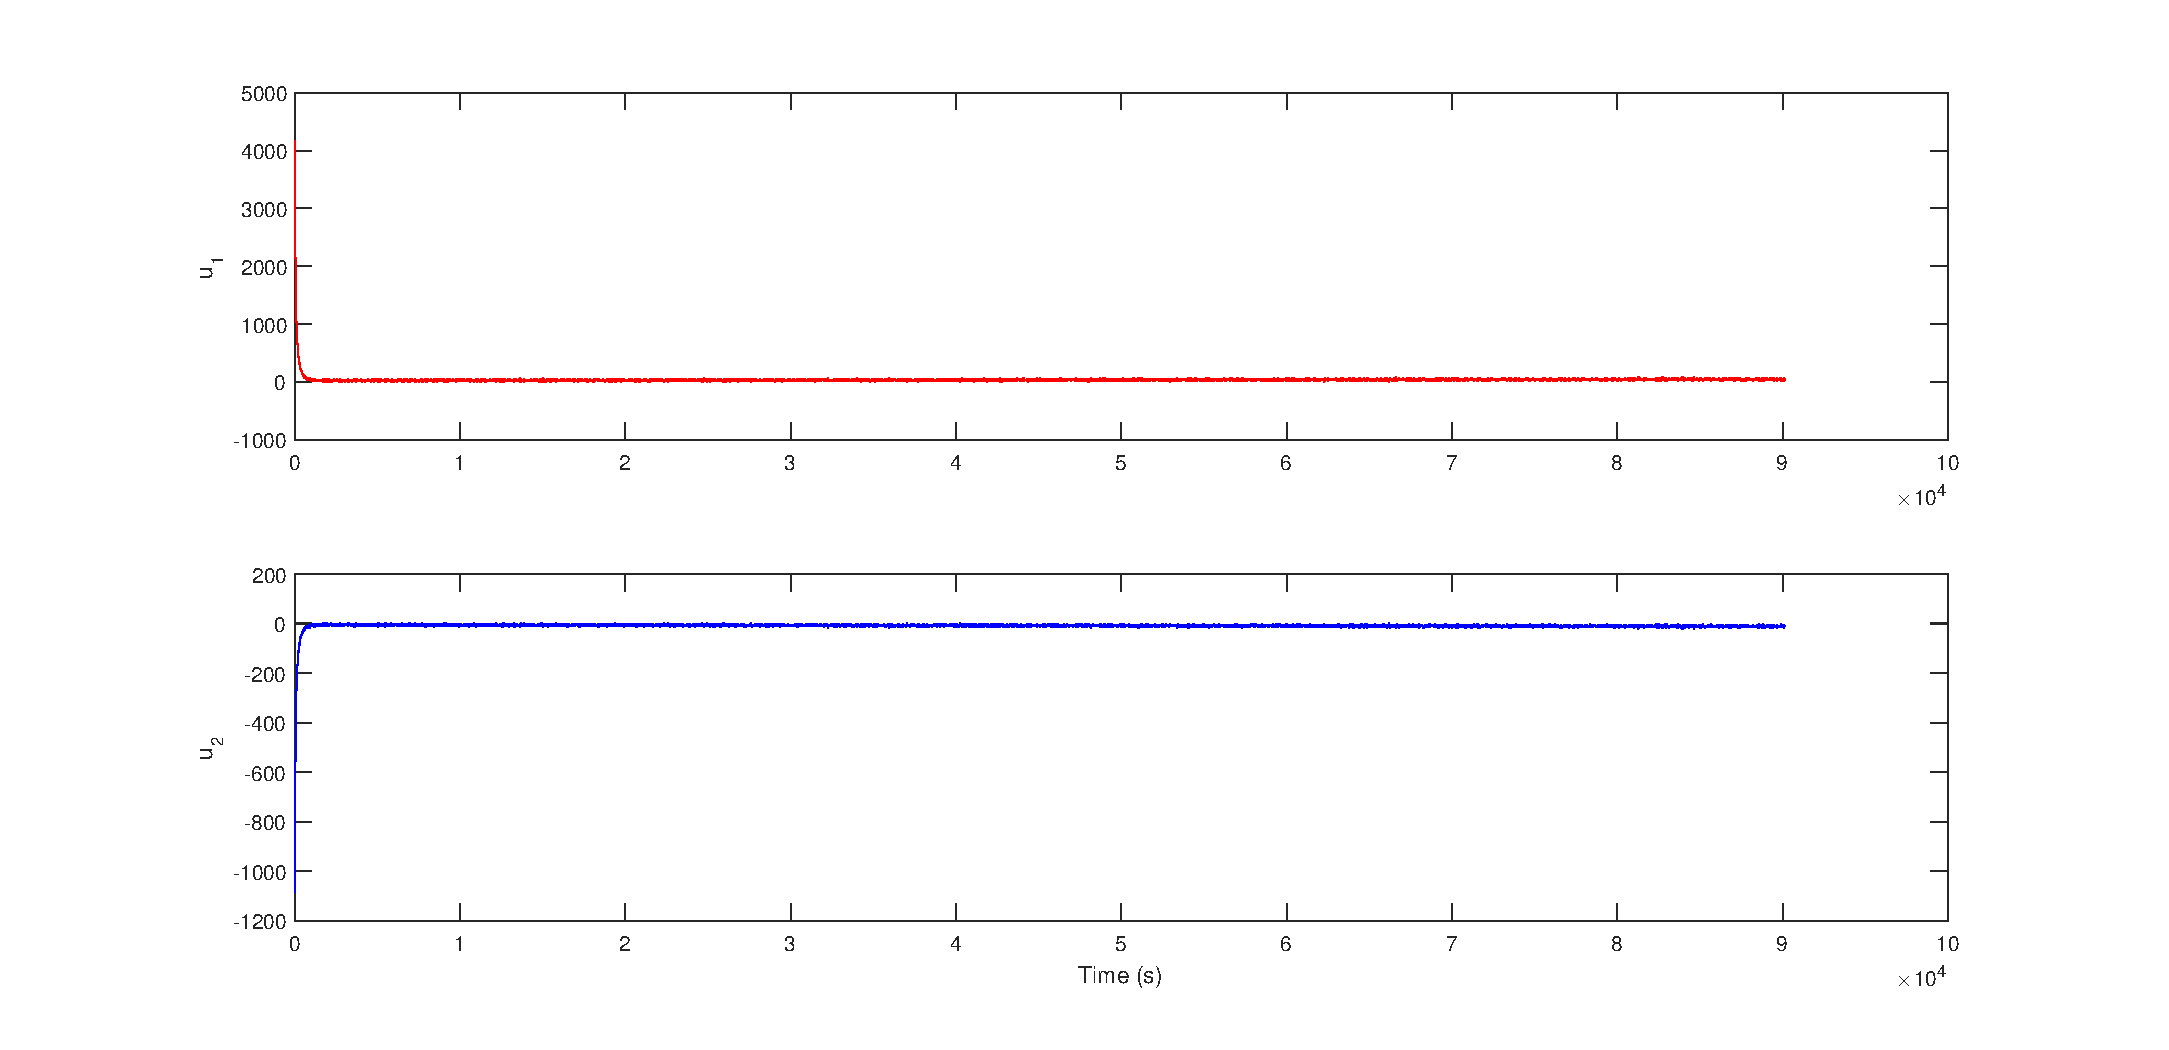
\includegraphics[width=0.5\paperwidth]{MatlabMain/results/whiteNoise/inputs}
\par\end{centering}
}\caption{\textbf{\emph{Constant set-point profile - Measurements with Gaussian
Noise: }}\emph{Here too the trend is the same, unaffected by addition
of noise. The last state reaches the set point. Second state still
has the same bias as seen previously.}}
\end{figure}


\subsection{Non Constant set-point profile}

\begin{table}[H]
\begin{centering}
\begin{tabular}{|c|c|}
\hline 
\textbf{Kalman Filter} & \textbf{Controller}\tabularnewline
\hline 
\hline 
$X_{0}=\begin{bmatrix}0.0472\\
-0.0576\\
-0.1655\\
-0.1065
\end{bmatrix}$ & p=7\tabularnewline
\hline 
$P_{0/0}=30000\times\begin{bmatrix}1 & 1 & 1 & 1\\
1 & 1 & 1 & 1\\
1 & 1 & 1 & 1\\
1 & 1 & 1 & 1
\end{bmatrix}$ & m=3\tabularnewline
\hline 
$Q=10e-3\times\begin{bmatrix}1 & 0 & 0 & 0\\
0 & 1 & 0 & 0\\
0 & 0 & 1 & 0\\
0 & 0 & 0 & 1
\end{bmatrix}$ & $Q_{y}=\begin{bmatrix}80 & 0 & 0\\
0 & 50 & 0\\
0 & 0 & 50
\end{bmatrix}$\tabularnewline
\hline 
$R=\begin{bmatrix}0.001 & 0 & 0\\
0 & 0.002 & 0\\
0 & 0 & 0.01
\end{bmatrix}$ & $Q_{u}=\begin{bmatrix}0.05 & 0\\
0 & 0.05
\end{bmatrix}$\tabularnewline
\hline 
\end{tabular}
\par\end{centering}
\caption{Tuned parameters}
\end{table}

\begin{figure}[H]
\begin{centering}
\subfloat[$C_{rc}$]{\begin{centering}
\includegraphics[scale=0.48]{\string"MatlabMain/results/whiteNoise/Non constant/Crc\string".pdf}
\par\end{centering}
}\subfloat[$O_{d}$]{\begin{centering}
\includegraphics[scale=0.48]{\string"MatlabMain/results/whiteNoise/Non constant/Od\string".pdf}
\par\end{centering}
}
\par\end{centering}
\centering{}\subfloat[$T_{rg}$]{\begin{centering}
\includegraphics[scale=0.48]{\string"MatlabMain/results/whiteNoise/Non constant/Trg\string".pdf}
\par\end{centering}
}\subfloat[Inputs]{\begin{centering}
\includegraphics[scale=0.48]{\string"MatlabMain/results/whiteNoise/Non constant/inputs\string".pdf}
\par\end{centering}
}\caption{\textbf{\emph{Non Constant set-point profile - Measurements with Gaussian
noise: }}\emph{This is similar to the case seen without noise. The
first state just crosses the set point and the other saturate without
approaching the set point themselves. It takes a lot of time for them
to cross to see what happens after that. It was not easy to speed
this up because large control inputs would lead to unstably high increments
crashing some optimisers.}}
\end{figure}


\section{Measurements with Fixed Bias}

\subsection{Constant set-point profile}

\begin{table}[H]
\begin{centering}
\begin{tabular}{|c|c|}
\hline 
\textbf{Kalman Filter} & \textbf{Controller}\tabularnewline
\hline 
\hline 
$X_{0}=\begin{bmatrix}0.0472\\
-0.0576\\
-0.1655\\
-0.1065
\end{bmatrix}$ & p=7\tabularnewline
\hline 
$P_{0/0}=30000\times\begin{bmatrix}1 & 1 & 1 & 1\\
1 & 1 & 1 & 1\\
1 & 1 & 1 & 1\\
1 & 1 & 1 & 1
\end{bmatrix}$ & m=3\tabularnewline
\hline 
$Q=10e-3\times\begin{bmatrix}1 & 0 & 0 & 0\\
0 & 1 & 0 & 0\\
0 & 0 & 1 & 0\\
0 & 0 & 0 & 1
\end{bmatrix}$ & $Q_{y}=\begin{bmatrix}4 & 0 & 0\\
0 & 5 & 0\\
0 & 0 & 5
\end{bmatrix}$\tabularnewline
\hline 
$R=\begin{bmatrix}0.001 & 0 & 0\\
0 & 0.002 & 0\\
0 & 0 & 0.01
\end{bmatrix}$ & $Q_{u}=\begin{bmatrix}0.05 & 0\\
0 & 0.05
\end{bmatrix}$\tabularnewline
\hline 
\end{tabular}
\par\end{centering}
\caption{Tuned parameters}
\end{table}

\begin{figure}[H]
\begin{centering}
\subfloat[$C_{rc}$]{\begin{centering}
\includegraphics[scale=0.45]{MatlabMain/results/bias/cons/Crc}
\par\end{centering}
}\subfloat[$O_{d}$]{\begin{centering}
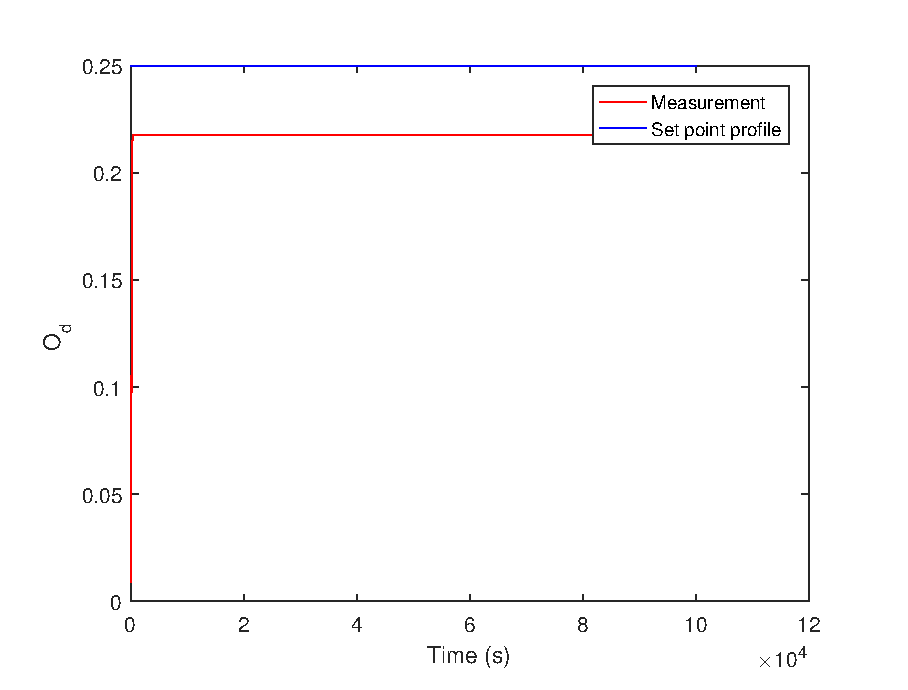
\includegraphics[scale=0.45]{MatlabMain/results/bias/cons/Od}
\par\end{centering}
}
\par\end{centering}
\centering{}\subfloat[$T_{rg}$]{\begin{centering}
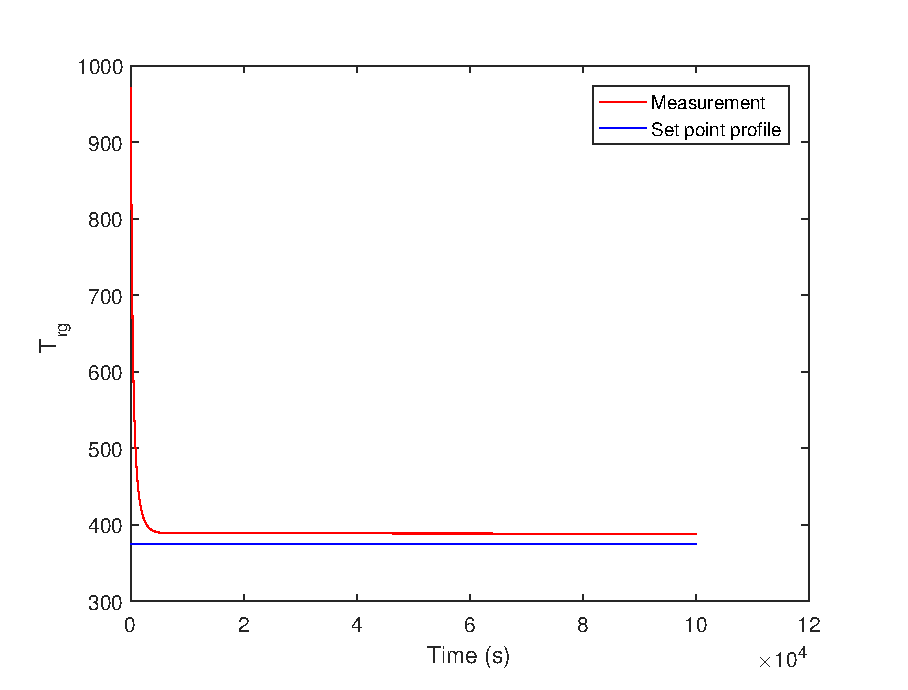
\includegraphics[scale=0.45]{MatlabMain/results/bias/cons/Trg}
\par\end{centering}
}\subfloat[Inputs]{\begin{centering}
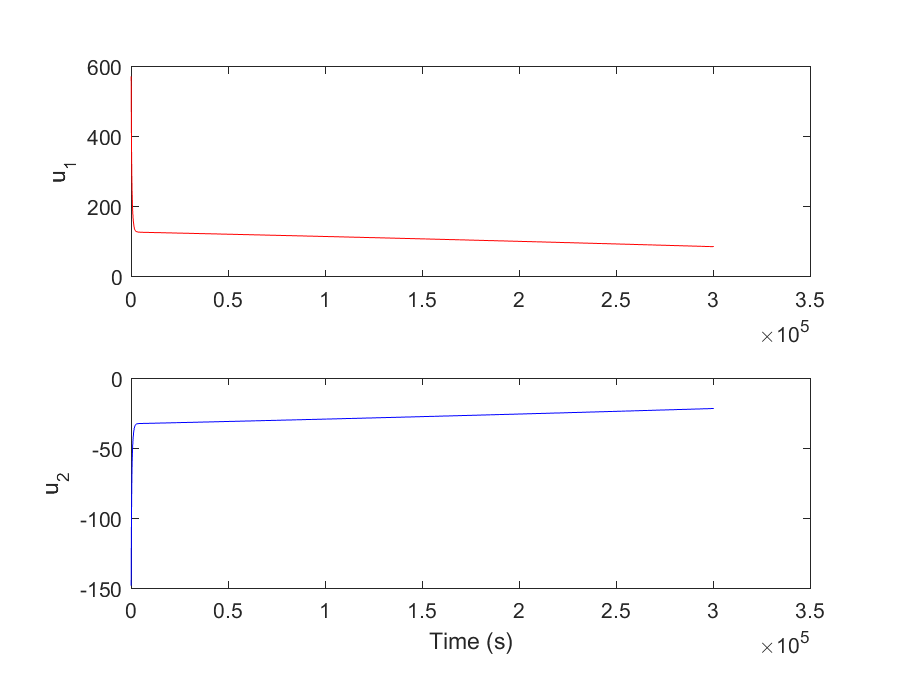
\includegraphics[scale=0.45]{MatlabMain/results/bias/cons/inputs}
\par\end{centering}
}\caption{\textbf{\emph{Non Constant set-point profile - Measurements with fixed
bias: }}\emph{As such the bias in measurents has not changed much
when the other cases are considered. The states still behave the same
way. The saturation values have changed a bit not directly related
to the bias. }}
\end{figure}


\subsection{Non Constant set-point profile}

\begin{table}[H]
\begin{centering}
\begin{tabular}{|c|c|}
\hline 
\textbf{Kalman Filter} & \textbf{Controller}\tabularnewline
\hline 
\hline 
$X_{0}=\begin{bmatrix}0.0472\\
-0.0576\\
-0.1655\\
-0.1065
\end{bmatrix}$ & p=7\tabularnewline
\hline 
$P_{0/0}=30000\times\begin{bmatrix}1 & 1 & 1 & 1\\
1 & 1 & 1 & 1\\
1 & 1 & 1 & 1\\
1 & 1 & 1 & 1
\end{bmatrix}$ & m=3\tabularnewline
\hline 
$Q=10e-3\times\begin{bmatrix}1 & 0 & 0 & 0\\
0 & 1 & 0 & 0\\
0 & 0 & 1 & 0\\
0 & 0 & 0 & 1
\end{bmatrix}$ & $Q_{y}=\begin{bmatrix}4 & 0 & 0\\
0 & 5 & 0\\
0 & 0 & 5
\end{bmatrix}$\tabularnewline
\hline 
$R=\begin{bmatrix}0.001 & 0 & 0\\
0 & 0.002 & 0\\
0 & 0 & 0.01
\end{bmatrix}$ & $Q_{u}=\begin{bmatrix}0.05 & 0\\
0 & 0.05
\end{bmatrix}$\tabularnewline
\hline 
\end{tabular}
\par\end{centering}
\caption{Tuned parameters}
\end{table}

\begin{figure}[H]
\begin{centering}
\subfloat[$C_{rc}$]{\begin{centering}
\includegraphics[scale=0.5]{\string"MatlabMain/results/bias/non cons/Crc\string".pdf}
\par\end{centering}
}\subfloat[$O_{d}$]{\begin{centering}
\includegraphics[scale=0.5]{\string"MatlabMain/results/bias/non cons/Od\string".pdf}
\par\end{centering}
}
\par\end{centering}
\centering{}\subfloat[$T_{rg}$]{\begin{centering}
\includegraphics[scale=0.5]{\string"MatlabMain/results/bias/non cons/Trg\string".pdf}
\par\end{centering}
}\subfloat[Inputs]{\begin{centering}
\includegraphics[scale=0.5]{\string"MatlabMain/results/bias/non cons/inputs\string".pdf}
\par\end{centering}
}\caption{\textbf{\emph{Non Constant set-point profile - Measurements with fixed
bias: }}\emph{Here too, the bias doesn't make much differemce. The
states behave the same way as before and don't reach the set point
on their own. }}
\end{figure}


\section{Variation in $X_{0}$ Control Horizon and Prediction Horizon}
\begin{itemize}
\item To understand the behaviour of the control system, a rigorous and
intensive parametric study is required, which is very time consuming. 
\item One trend is that for a very high p=45, m = 40, the bias in $T_{rg}$
is removed. But again beyond some point, it departs from the set point.
However, the other two states doesn't seem to converge to setpoint
within this time. If for the same case, m is reduced to 10, $T_{rg}$
stays at the set point reasonably. Even here, the other states don't
converge.
\item A significant change is not seen by varying m, p in small steps.
\end{itemize}
\begin{figure}[H]
\begin{centering}
\subfloat[p=45,m=40]{\begin{centering}
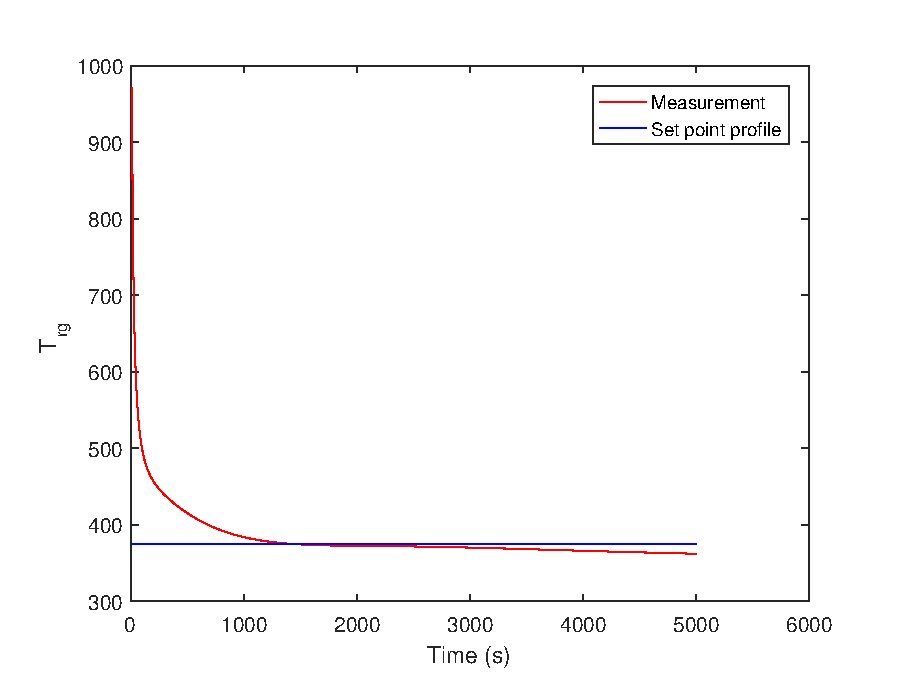
\includegraphics[scale=0.5]{MatlabMain/results/horizon/m40p45/Trg}
\par\end{centering}
}\subfloat[p=45, m=10]{\begin{centering}
\includegraphics[scale=0.5]{\string"MatlabMain/results/horizon/m40p45 - Copy/Trg\string".pdf}
\par\end{centering}
}
\par\end{centering}
\centering{}\caption{\textbf{\emph{Behaviour of m,p}}}
\end{figure}

\begin{figure}[H]
\begin{centering}
\subfloat[p=45,m=40]{\begin{centering}
\includegraphics[scale=0.5]{MatlabMain/results/horizon/m40p45/Crc}
\par\end{centering}
}\subfloat[p=45, m=10]{\begin{centering}
\includegraphics[scale=0.5]{\string"MatlabMain/results/horizon/m40p45 - Copy/Crc\string".pdf}
\par\end{centering}
}
\par\end{centering}
\centering{}\caption{\textbf{\emph{Behaviour of m,p}}}
\end{figure}

\begin{figure}[H]
\begin{centering}
\subfloat[p=45,m=40]{\begin{centering}
\includegraphics[scale=0.5]{MatlabMain/results/horizon/m40p45/Od}
\par\end{centering}
}\subfloat[p=45, m=10]{\begin{centering}
\includegraphics[scale=0.5]{\string"MatlabMain/results/horizon/m40p45 - Copy/Od\string".pdf}
\par\end{centering}
}
\par\end{centering}
\centering{}\caption{\textbf{\emph{Behaviour of m,p}}}
\end{figure}

\begin{itemize}
\item The trends with $X_{0}$ is shown in the following figures.
\end{itemize}
\begin{figure}[H]
\begin{centering}
\subfloat[$C_{rc}$]{\begin{centering}
\includegraphics[scale=0.5]{MatlabMain/results/X0/0.3X0/Crc}
\par\end{centering}
}\subfloat[$O_{d}$]{\begin{centering}
\includegraphics[scale=0.5]{MatlabMain/results/X0/0.3X0/Od}
\par\end{centering}
}
\par\end{centering}
\centering{}\subfloat[$T_{rg}$]{\begin{centering}
\includegraphics[scale=0.5]{MatlabMain/results/X0/0.3X0/Trg}
\par\end{centering}
}\subfloat[Inputs]{\begin{centering}
\includegraphics[scale=0.5]{MatlabMain/results/X0/0.3X0/Trg}
\par\end{centering}
}\caption{\textbf{\emph{X0={[} 0.0354 -0.0432 -0.1241 -0.0798{]}: }}\emph{The
first state approches set point very slowly. It was not possible to
increase it's approach rate even with very high weights. Second state
comes closer and then moves away from the set point. It takes a saturated
value it was always reaching. The third state just departs from the
set point which is unusual. May further tuning could have alleviated
this issue. }}
\end{figure}

\begin{figure}[H]
\begin{centering}
\subfloat[$C_{rc}$]{\begin{centering}
\includegraphics[scale=0.5]{\string"MatlabMain/results/X0/0.3X0 - Copy/Crc\string".pdf}
\par\end{centering}
}\subfloat[$O_{d}$]{\begin{centering}
\includegraphics[scale=0.5]{\string"MatlabMain/results/X0/0.3X0 - Copy/Od\string".pdf}
\par\end{centering}
}
\par\end{centering}
\centering{}\subfloat[$T_{rg}$]{\begin{centering}
\includegraphics[scale=0.5]{\string"MatlabMain/results/X0/0.3X0 - Copy/Trg\string".pdf}
\par\end{centering}
}\subfloat[Inputs]{\begin{centering}
\includegraphics[scale=0.5]{\string"MatlabMain/results/X0/0.3X0 - Copy/inputs\string".pdf}
\par\end{centering}
}\caption{\textbf{\emph{X0={[} 0.0402 -0.0490 -0.1407 -0.0905{]}: }}\emph{This
is even closer to the set point. Strangely, the system is not able
to achieve the set point. The states behave the same way. }}
\end{figure}


\section{Conclusions}
\begin{itemize}
\item Only the third state seems to be reasonably controllable and stable
by suitably choosing large p and m. It can be made to stay at the
desired set point.
\item Second state always had an offset which could not be removed. By studying
this bias variation and it's consequences, we can may be define a
new state with this bias subtracted. 
\item First state was always increasing and it was never possible to saturate
it. May be a threshold can be set. But essentially, it is possible
to take the state to desired set point, but it cannot be made to stay
there. So. technocally, it is ``Controllable''.
\item Even if the system started from somewhere near the set point, the
second state digresses to reach it's steady value. The third state
completely diverges from the reference. First state just increases
almost linearly as it always did.
\item It has to be noted that the bias may be because the controller and
the Kalman filter work on the linearized model. The non linear model
can be implemented if it's really important to fix these issues. But
then again, it's a tradeoff between calulation time and system performance. 
\end{itemize}

\end{document}
